\documentclass[11pt,a4paper]{article}
\usepackage[utf8]{inputenc}
\usepackage{amsfonts}
\usepackage{pdfpages}
\usepackage{eurosym}
\usepackage{pgfplots}
\usepackage{authblk}
\usepackage{url}
\usepackage{multirow}
\usepackage{booktabs}
\usepackage{float}
\usepackage{listings}

\usepackage{hyperref}
\hypersetup{
    colorlinks=true,
    linkcolor=black,
    filecolor=magenta,      
    urlcolor=cyan,
    pdftitle={Overleaf Example},
    pdfpagemode=FullScreen,
    }
\usepackage{algpseudocode}
\usepackage{algorithm}
\usepackage{letltxmacro}
\usepackage{microtype}
\usepackage[left=3cm,right=3cm,bottom=3.5cm]{geometry}
\usepackage{emptypage}
\usepackage{amsmath,amssymb,amsthm, latexsym}
\usepackage[english,italian]{babel}
\usepackage{url}
\usepackage{caption}
\usepackage{verbatim}
\captionsetup{tableposition=top,figureposition=bottom,font=small,format=hang,labelfont={sf,bf}}
\usepackage{graphicx}
\usepackage{tabularx}
\usepackage{listings}
\usepackage{hyphenat}
\usepackage{subfig}
\pagestyle{empty}
\newcommand\AlCentroPagina[1]{%
\AddToShipoutPicture*{\AtPageCenter{%
\makebox(0,0){\includegraphics%
[width =0.9\paperwidth]{#1}}}}}

\begin{document}
\newcommand{\horrule}[1]{\rule{\linewidth}{#1}}
\lstset{language=Java} 
\lstset{basicstyle=\footnotesize\ttfamily}
\author{Silvio Baratto, Tobias Ganzmann}
\title{
\normalfont \normalsize 
\href{https://github.com/SilvioBaratto/Numerical-and-Data-Intensive-Computing}{github.com/SilvioBaratto/Lab-1} \\ [25pt] % Your university, school and/or department name(s)
\horrule{0.5pt} \\[0.4cm] % Thin top horizontal rule
\huge Report Lab 1\\ % The assignment title
\horrule{2pt} \\[0.5cm] % Thick bottom horizontal rule
}
\maketitle
\tableofcontents
\newpage
\section{PERF (I)}
\subsection{Definition profiler}
A profiler in software engineering, is a form of dynamic program analysis that measures, for example, the space (memory) or time complexity of a program, the usage of particular instructions, or the frequency and duration of function calls. Most commonly, profiling information serves to aid program optimization, and more specifically, performance engineering. Profilers, which are also programs themselves, analyze target programs by collecting information on their execution. Based on their data granularity, on how profilers collect information, they are classified into event based or statistical profilers.\\
\subsection{Code explanatin for benchmarking}
The code given to do some performance analysis using perf as a profiler consist in a simple function that initialize a matrix of dimension $2000 \times 2000$ and fill all the matrix with a value equal to $1$. The program repeat this operation $100$ times. 
\subsection{Performance analysis tool (perf)}
We are interested in see how the program behaves with different optimizers and code optimizations using perf to check the performance results. To do that with this instructions we want to look at:
\begin{itemize}
\item[\textbf{a.}] CPU clock cycles at user level
\item[\textbf{b.}] Machine code instructions at user level
\item[\textbf{c.}] First-level data cache load hitst at user level
\item[\textbf{d.}] First-level data cache load misses at user level
\item[\textbf{e.}] First-level data cache store hits at user level
\item[\textbf{f.}] First-level data cache store misses at user level
\item[\textbf{g.}] Last-level cache load hits at user level
\item[\textbf{h.}] Last-level cache load misses at user level
\item[\textbf{i.}] Last-level cache store hits at user level
\item[\textbf{j.}] Last-level cache store misses at user level
\end{itemize}
The way how we obtain the following benchmark results is from this terminal command:
\begin{lstlisting}[language=bash]
  $ sudo perf stat -e cycles:u -e instructions:u \
                	-e L1-dcache-loads:u -e L1-dcache-load-misses:u \
                	-e L1-dcache-stores:u -e L1-dcache-store-misses:u \
                	-e LLC-loads:u -e LLC-load-misses:u \
                	-e LLC-stores:u -e LLC-store-misses:u ./task1 
\end{lstlisting}
From the first run of the code we obtain the following results:
\begin{lstlisting}[language=bash]
CPU = 5.893150 ms 

 Performance counter stats for './task1':

     2,743,735,005      cycles:u         	  (32.74%)
     3,199,246,694      instructions:u            (44.26%)
       402,366,995      L1-dcache-loads           (55.79%)
       803,099,963      L1-dcache-load-misses     (67.31%)
       799,527,269      L1-dcache-stores          (67.46%)
   <not supported>      L1-dcache-store-misses                                      
         1,628,527      LLC-loads                 (67.46%)
             1,094      LLC-load-misses           (44.21%)
         2,479,174      LLC-stores                (21.69%)
               258      LLC-store-misses          (21.69%)

       0.590644181 seconds time elapsed

       0.590584000 seconds user
       0.000000000 seconds sys
\end{lstlisting}
Changing the code in such way that array is now traversed by rows
instead of by columns, hence taking advantage of both the row major order used in C and the cache hierarchy we obtain the following results:
\begin{lstlisting}[language=bash]
CPU = 1.423880 ms 

 Performance counter stats for './task1':

       648,114,804      cycles:u                  (32.97%)
     1,624,440,721      instructions:u            (44.14%)
       396,820,828      L1-dcache-loads           (55.31%)
        12,204,130      L1-dcache-load-misses     (66.48%)
       383,946,246      L1-dcache-stores          (66.48%)
   <not supported>      L1-dcache-store-misses                                      
             1,680      LLC-loads                 (66.48%)
                40      LLC-load-misses           (44.69%)
         6,988,534      LLC-stores                (22.35%)
                67      LLC-store-misses          (22.35%)

       0.143955657 seconds time elapsed

       0.135983000 seconds user
       0.007999000 seconds sys
\end{lstlisting}
\subsection{Conclusion}
From the following graphs we can see the results of the different optimization methods and the comparison between normal matrix calcuation and row-major-ordering used in C. As can be shown, the cycles and instructions are much smaller in the when using both optimization approaches in comparison to the initial approach. \\
We observe similar results in the usage of L1-cache with an exception of the load misses, which are less frequent in row-major-version of the program in general.\\
Looking at llc\_flow behaviour, we see an improvement in llc\_loads with row-major-ordering, however llc\_stores are increased.
\begin{figure}[h]
\centering
\subfloat[]
  {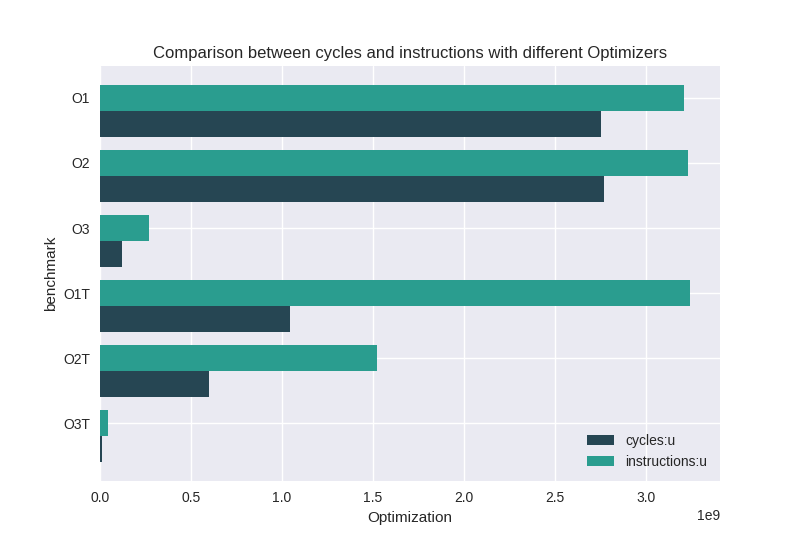
\includegraphics[width=.5\textwidth]{foto/cycles_and_instructions.png}}\hfill
\subfloat[]
  {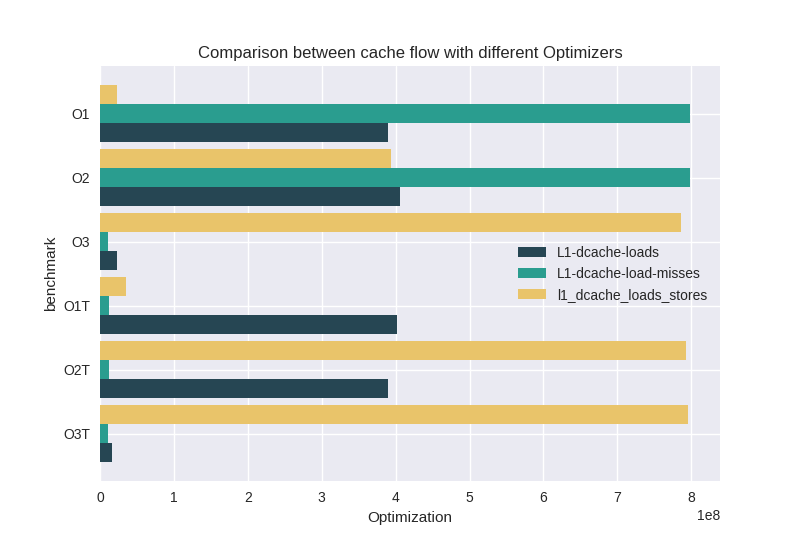
\includegraphics[width=.5\textwidth]{foto/cache_flow_comparison.png}}\hfill
\subfloat[]
  {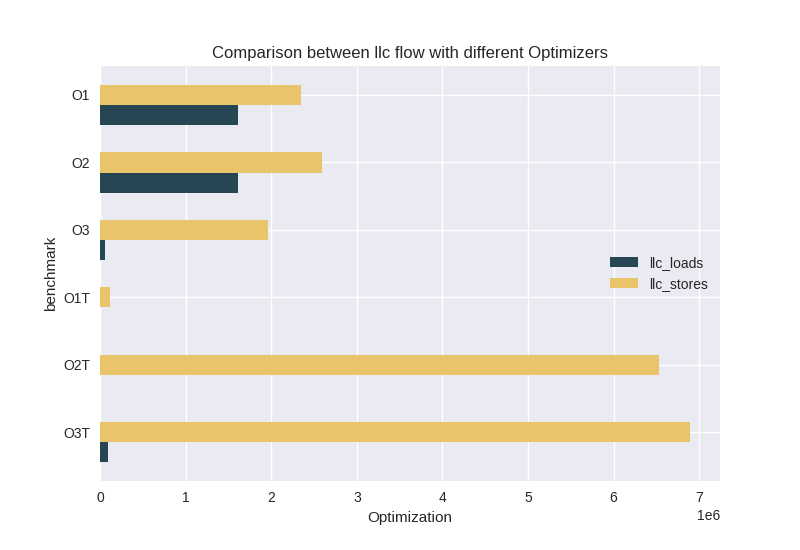
\includegraphics[width=.5\textwidth]{foto/llc_comparison.png}}
\end{figure}

\newpage
\section{PERF (II)}
The program given initializes two random matrices. The first part performs simple matrix multiplication without taking advantage of the row-major order used in C and the cache hierarchy. We analyze the performance of this approach:
\subsection{Program without optimization}
\begin{lstlisting}[language=bash]
CPU = 655.932007 ms Mul1 

 Performance counter stats for './task2':

     6,065,174,592      cycles:u                  (33.25%)
    18,111,358,969      instructions:u            (44.57%)
     4,031,509,126      L1-dcache-loads           (55.85%)
     2,034,376,280      L1-dcache-load-misses     (66.88%)
     2,017,118,230      L1-dcache-stores          (66.88%)
   <not supported>      L1-dcache-store-misses                                      
           708,795      LLC-loads                 (66.89%)
             3,761      LLC-load-misses           (44.15%)
           429,307      LLC-stores                (22.08%)
            53,142      LLC-store-misses          (22.07%)

       1.413953736 seconds time elapsed

       1.409785000 seconds user
       0.004005000 seconds sys
\end{lstlisting}
Afterwards we apply said optimization towards more beneficial calculation order (and check for correctness, of course) and run the performance analysis again:
\subsection{Program with optimization}
\begin{lstlisting}[language=bash]
CPU = 664.648987 ms Mul1 

 Performance counter stats for './task2':

     6,148,114,191      cycles:u                 (33.03%)
    18,299,920,676      instructions:u           (44.29%)
     4,060,471,919      L1-dcache-loads          (55.58%)
     2,035,551,933      L1-dcache-load-misses    (66.82%)
     2,010,732,108      L1-dcache-stores         (67.10%)
   <not supported>      L1-dcache-store-misses                                      
           563,053      LLC-loads                (67.10%)
             4,433      LLC-load-misses          (44.42%)
           468,321      LLC-stores               (21.93%)
            65,307      LLC-store-misses         (21.93%)

       1.350588624 seconds time elapsed

       1.346580000 seconds user
       0.004007000 seconds sys
\end{lstlisting}
Overall, no significant improvement can be seen (1.41s versus 1.35s). The main difference can be observed in LLC-loads. 
\newpage
\section{GPROF}
\subsection{self-explained "profile" file}
This file provide benchmarks of all the function runned by the program \texttt{algi.c}, giving the the percentage of the total running time of the time program used by one function, the number of seconds accounted for by one function alone and the average number of milliseconds spent in this ms/call function per call.
\subsection{Bottlenecks and best candidates to parallelized}
\begin{itemize}
\item[a] Functions with high "self ms/call" (shown in green) values and a big percentage of running time are considered our bottlenecks. The cannot be divided into smaller pieces and therefore not be parallelized.
\item[b] In contrast, functions with low "self ms/call" (shown in blue) values and frequent calls are already divided up in small, very managable chunks and can therefore be parallelized. In this case we divide the matrices in chunks and loop over them seperately in parallel (for example domain decomposition).
\end{itemize}
\begin{figure}[h]
\centering
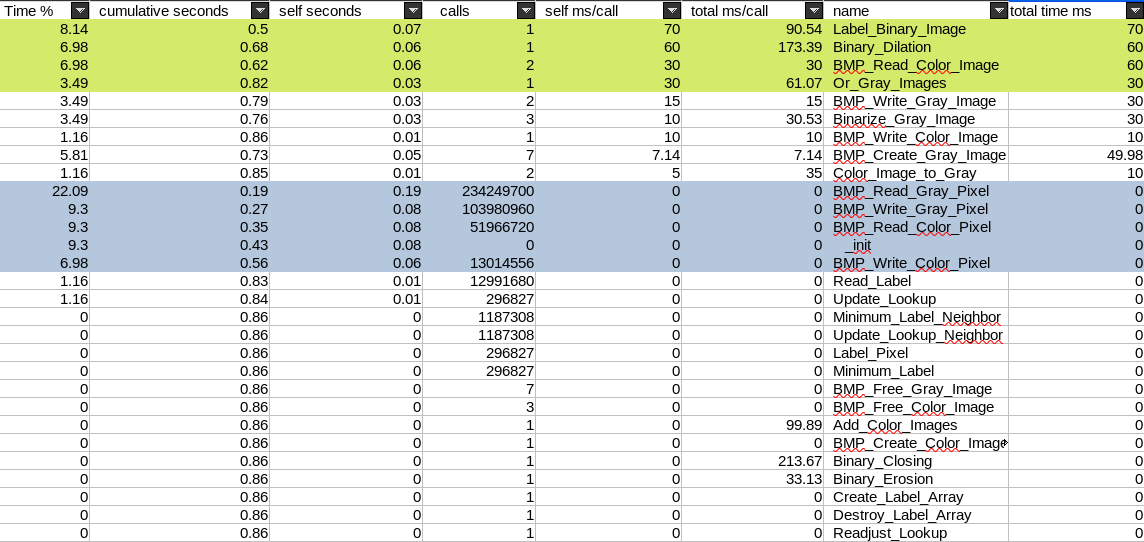
\includegraphics[width=\textwidth]{foto/calls.png}
\end{figure}
\newpage
\section{OpenMP (Compilation and basic directives)}
\subsection{CPU information from the Linux kernel}
\begin{lstlisting}[language=bash]
model name	: 11th Gen Intel(R) Core(TM) i7-1165G7 @ 2.80GHz

processor	: 0, physical id 0
processor	: 1, physical id 0
processor	: 2, physical id 0
processor	: 3, physical id 0
processor	: 4, physical id 0
processor	: 5, physical id 0
processor	: 6, physical id 0
processor	: 7, physical id 0

cpu cores	: 4
siblings	: 8

processor	: 0, physical id:	0, core id: 0
processor	: 1, physical id:	0, core id: 1
processor	: 2, physical id:	0, core id: 2
processor	: 3, physical id:	0, core id: 3
processor	: 4, physical id:	0, core id: 0
processor	: 5, physical id:	0, core id: 1
processor	: 6, physical id:	0, core id: 2
processor	: 7, physical id:	0, core id: 3
\end{lstlisting}
\subsection{Number of cores and threads from internet}
In the \href{https://ark.intel.com/content/www/es/es/ark/products/208662/intel-core-i71165g7-processor-12m-cache-up-to-4-70-ghz.html}{intel} website we can find the same information:
\begin{figure}[h]
\centering
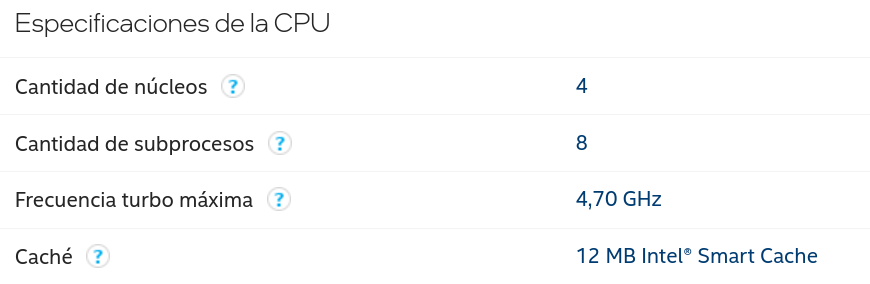
\includegraphics[width=0.8\textwidth]{foto/intel.png}
\end{figure}
\subsection{Program explanation}
Task1 is a simple for loop iterating 2 billion times and counting up two variables, j as a long datatype and k as a double datatype. 
In accordance with the task description we run the program under different conditions: 1 thread, 2 threads, 2 threads but limited to one CPU, 4 threads.
\subsection{Benchmarks with multiple threads}
Analyzing the behaviour with gnome system monitor we can see spikes in utilization of the cores, depending on usage. With altering the number of threads we allow the program to run on more than one CPU, resulting in significant speedup of the total execution time (see SpeedUp in table and blue line in graph. What can also be observed on the other hand is actually a decrease in efficiency with an increase of speedup, due to CPU timing, coordination and communication between processing units.
\begin{figure}[h]
\centering
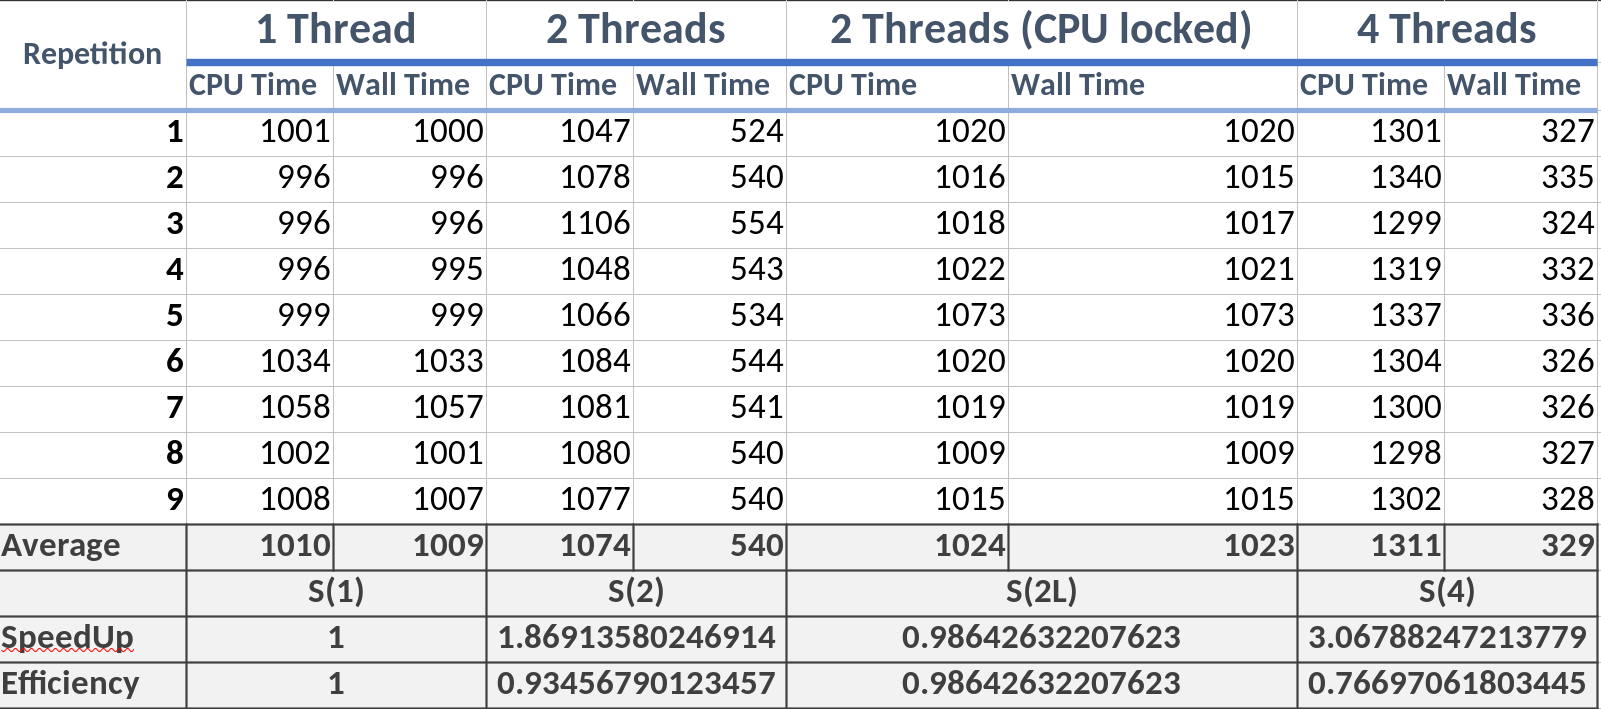
\includegraphics[width=\textwidth]{foto/times.png}
% 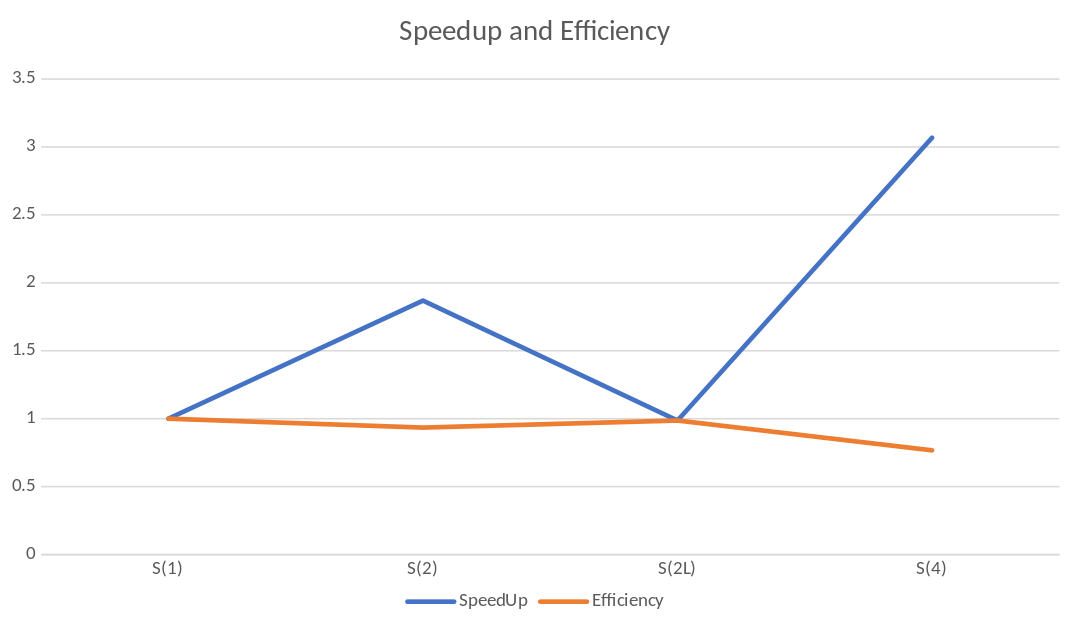
\includegraphics[width=\textwidth]{foto/speedup.png}
\end{figure}
\subsection{Speedup and Efficiency}
\begin{figure}[h]
\centering
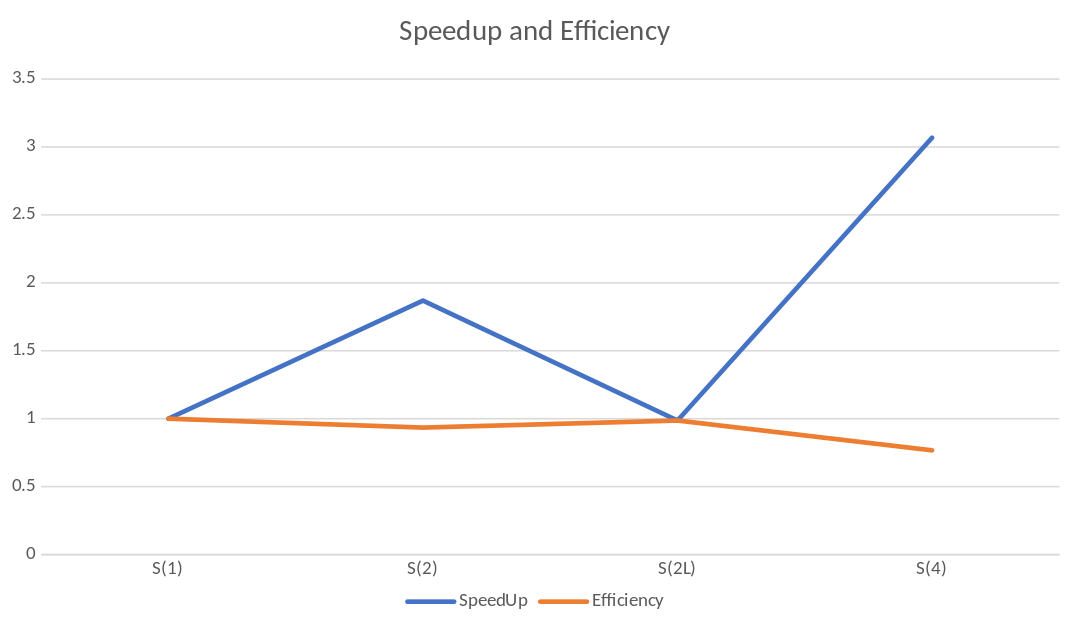
\includegraphics[width=\textwidth]{foto/speedup.png}
\end{figure}
\subsection{Task 2 program explanation}
The program task 2 creates a big random number "limit" and iterates "limit" times to increase the variable j by 1 for each loop in a parallel environment.The output of the program gives us the value of j for each thread used. 
\subsection{Program behaviour}
We observe that the the order of the execution of the threads as well as the starting thread PID is not constant but changes every execution. This does not change when setting the PID variable to private, even though, now every thread used it's own private copy of the variable. The reason for this is, that in the given program the PID variable is not actually being used for anything but giving the overview.
\subsection{Changing from "private" to "firstprivate"}
Now we take a look at the initialization of the "limit" variable. In the master thread the variable is initally set to -1, however, with being set to private in the parallel part, it is re-initialized for every parallel thread to 0. Changing the variable to firstprivate results in the initial value being kept even in the parallel threads.
\newpage
\section{Optional assignment}
\subsection{Program task 3 explanation}
The program task 3 creates a parallel enviroment with 2 threads. The program has two workloads that behave in the same way (1000 loops, count up everz 10th loop, looped 10 times).
\subsection{Behaviour semaphores}
As shown in the image with the semaphores the thread that arrives first has the precedence and the other must wait the execution of the first one. When the first thread ends its task the second one can execute the workload. This is the reason why they run alternately. 
\begin{figure}[h]
\centering
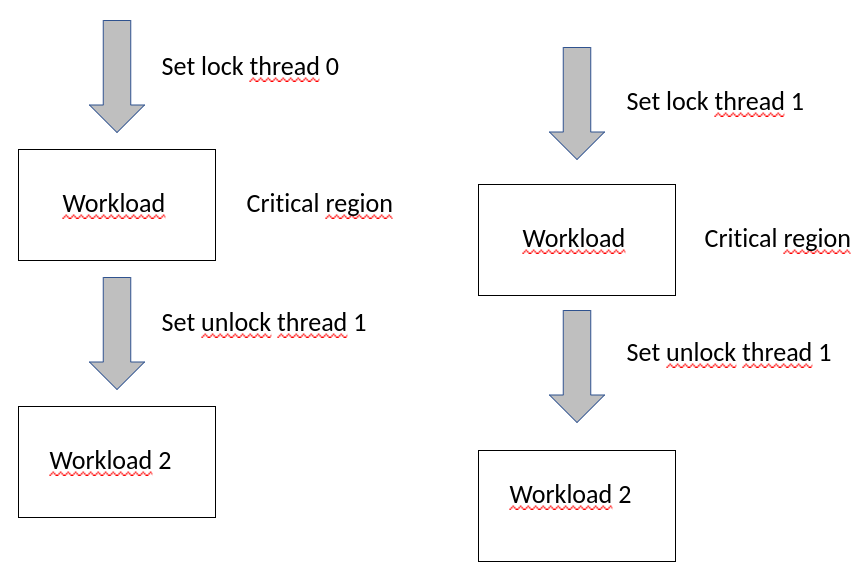
\includegraphics[width=0.5\textwidth]{foto/sem_explanation.png}
\end{figure}
\subsection{Comment omp lock and omp unlock}
If we comment the omp\_set\_lock and omp\_set\_unlock the program doesn't behave in the same way because we remove the "precedence" we create before using sempahores. So every thread execute could execute the workload in the same moment. \\
If we use the command "\#pragma omp critical" we obtain the same results as using sempahores. A critical region behaves as semaphores, creating precedence between threads and so the workload can not be execute in the same moment by different threads. 
\subsection{Inserting barrier synchronization}
Barrier block everythread before the workload and decide who goes first as shown in this picture.
\begin{figure}[h]
\centering
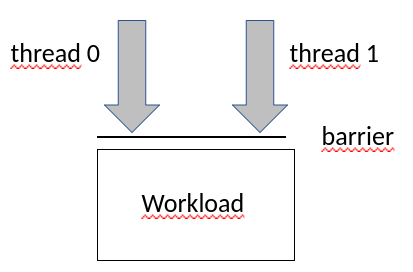
\includegraphics[width=0.3\textwidth]{foto/barrier.png}
\end{figure}
If we comment omp\_unset\_lock we remove the option for the lock to be opened again, resulting in the program being stuck after the first iteration of the first thread. \\
A similar problem arises with the use of the barrier inside of the lock. As the barrier waits for all threads to be finished with the current task, the program gets stuck, because the semaphore does not allow the second thread to enter into the workload.
\subsection{task 4}
The result of the calculation is wrong because both threads are trying to increase the shared variable k at the same the. This results in the variale being increased by 1 twice for each time the loop runs, thus making the result only half of the correct answer. \\
Introducing the reduction clause splits the workload to two separate private variables and combines them after the loop is done, resulting in the correct answer.
\end{document}